%%%%%%%%%%%%%%%%%%%%%%% Boundary-Layer Meteorology 2019 Template %%%%%%%%%%%%%%%%%%%%%%%%%

%  ══════════════════════════════════════════════════════════════════════════
% packages
\RequirePackage{fix-cm}
\documentclass[smallextended]{svjour3}       
\smartqed  
\usepackage{appendix}
\usepackage{amsmath}
\usepackage{graphicx}
\usepackage{lineno}
\usepackage{array}
\usepackage{longtable}
\usepackage{natbib}
\setcitestyle{aysep={}}
\linenumbers

\newcommand*\patchAmsMathEnvironmentForLineno[1]{%
\expandafter\let\csname old#1\expandafter\endcsname\csname #1\endcsname
\expandafter\let\csname oldend#1\expandafter\endcsname\csname end#1\endcsname
\renewenvironment{#1}%
{\linenomath\csname old#1\endcsname}%
{\csname oldend#1\endcsname\endlinenomath}}% 
\newcommand*\patchBothAmsMathEnvironmentsForLineno[1]{%
\patchAmsMathEnvironmentForLineno{#1}%
\patchAmsMathEnvironmentForLineno{#1*}}%
\AtBeginDocument{%
\patchBothAmsMathEnvironmentsForLineno{equation}%
\patchBothAmsMathEnvironmentsForLineno{align}%
\patchBothAmsMathEnvironmentsForLineno{flalign}%
\patchBothAmsMathEnvironmentsForLineno{alignat}%
\patchBothAmsMathEnvironmentsForLineno{gather}%
\patchBothAmsMathEnvironmentsForLineno{multline}%
}
%  ══════════════════════════════════════════════════════════════════════════


\begin{document}


%  ══════════════════════════════════════════════════════════════════════════
% title
%  ══════════════════════════════════════════════════════════════════════════

\title{Evidence of a Shear Driven Gravity Wave within the formation of a Stable Boundary Layer}


%  ══════════════════════════════════════════════════════════════════════════
% authors
%  ══════════════════════════════════════════════════════════════════════════

\author{
Douglas Keller \and
Sneha Ramakrishnan \and
Dishi Thomas \and
Elsa Dieudonné \and
Antonio Donateo \and
Natalie Brett \and
Brice Barret \and
Roman Pohorsky \and
Slimane Bekki \and
Jean-Christophe Raut \and
Julia Schmale \and
Kathy S. Law \and
Steve R. Arnold \and
William R. Simpson \and
Stefano Decesari \and
Gilberto Javier Fochesatto
}

\institute{
    D. Keller \at
    Laboratoire de Météorologie Dynamique, École Polytechnique, Institute Polytechnique de Paris, Palaiseau, FR \\
    \email{dg.kllr.jr@gmail.com} 
    \and
    S. Ramakrishnan \at
    Department of Atmospheric Sciences, University of Alaska Fairbanks, Fairbanks, Alaska, USA \\
    \and
    D. Thomas \at
    Department of Atmospheric Sciences, University of Alaska Fairbanks, Fairbanks, Alaska, USA \\
    \and
    E. Dieudonné \at
    Laboratoire de Physico-Chimie de l’Atmosphère, Université du Littoral Côte d’Opale, Dunkerque, FR \\
    \and
    A. Donateo \at
    National Research Council of Italy, Institute of Atmospheric Sciences and Climate (CNR-ISAC), Lecce, IT \\
    \and
    N. Brett \at
    Sorbonne Université, UVSQ, CNRS, LATMOS, Paris, FR \\
    \and
    B. Barret \at
    Laboratoire d’Aérologie (LAERO), Université Toulouse III – Paul Sabatier, CNRS, Toulouse, FR \\
    \and
    R. Pohorsky \at
    Extreme Environments Research Laboratory. Ecole Polytechnique Fédérale de Lausanne, Sion, CH \\
    \and
    S. Bekki \at
    Sorbonne Université, UVSQ, CNRS, LATMOS, Paris, FR \\
    \and
    J.-C. Raut \at
    Sorbonne Université, UVSQ, CNRS, LATMOS, Paris, FR \\
    \and
    J. Schmale \at
    Extreme Environments Research Laboratory. Ecole Polytechnique Fédérale de Lausanne, Sion, CH \\
    \and
    K. Law \at
    Sorbonne Université, UVSQ, CNRS, LATMOS, Paris, FR \\
    \and
    S. Arnold \at
    School of Earth and Environment, University of Leeds, Leeds, LS2 9JT, UK \\
    \and
    W. Simpson \at
    Department of Chemistry. University of Alaska Fairbanks, Fairbanks, Alaska, USA \\
    \and
    S. Decesari \at
    National Research Council of Italy, Institute of Atmospheric Sciences and Climate (CNR-ISAC), Lecce, IT \\
    \and
    G. Fochesatto \at
    Department of Atmospheric Sciences, University of Alaska Fairbanks, Fairbanks, Alaska, USA \\
}

\date{Received: DD Month YEAR / Accepted: DD Month YEAR}

\maketitle


%  ══════════════════════════════════════════════════════════════════════════
% abstract
%  ══════════════════════════════════════════════════════════════════════════

\begin{abstract} % 250 words
In February 2022, during the ALPACA campaign at the University of Alaska Fairbanks, instruments captured a gravity wave embedded in a stable surface-based temperature inversion layer (SBI) during a shallow cold flow (SCF) event. Doppler lidar, microwave radiometer, and sonic anemometer data show that the SCF extended from the surface to ~100 m, generating shear instability (gradient Richardson number Rg< 0.5) within the SBI. The main wave signal occurred near 150 m, with dominant frequencies of one cycle over 38 to 50 minutes, far lower than the local Brunt–Väisälä frequency, indicating a wave-driven process. Continuous wavelet analysis revealed maximum energy at the shear interface. Moreover, a secondary wave approaching from above (~300 m) was documented, connected to unstable layers present between 750–1000 m. These observations provide new insight into wave–shear interactions in stable Arctic boundary layers.
\end{abstract}


%  ══════════════════════════════════════════════════════════════════════════
% introduction
%  ══════════════════════════════════════════════════════════════════════════

\section{Introduction}
\label{intro}

Gravity Waves
Shallow Cold Flow
ALPACA Campaign

\begin{figure}
\centering
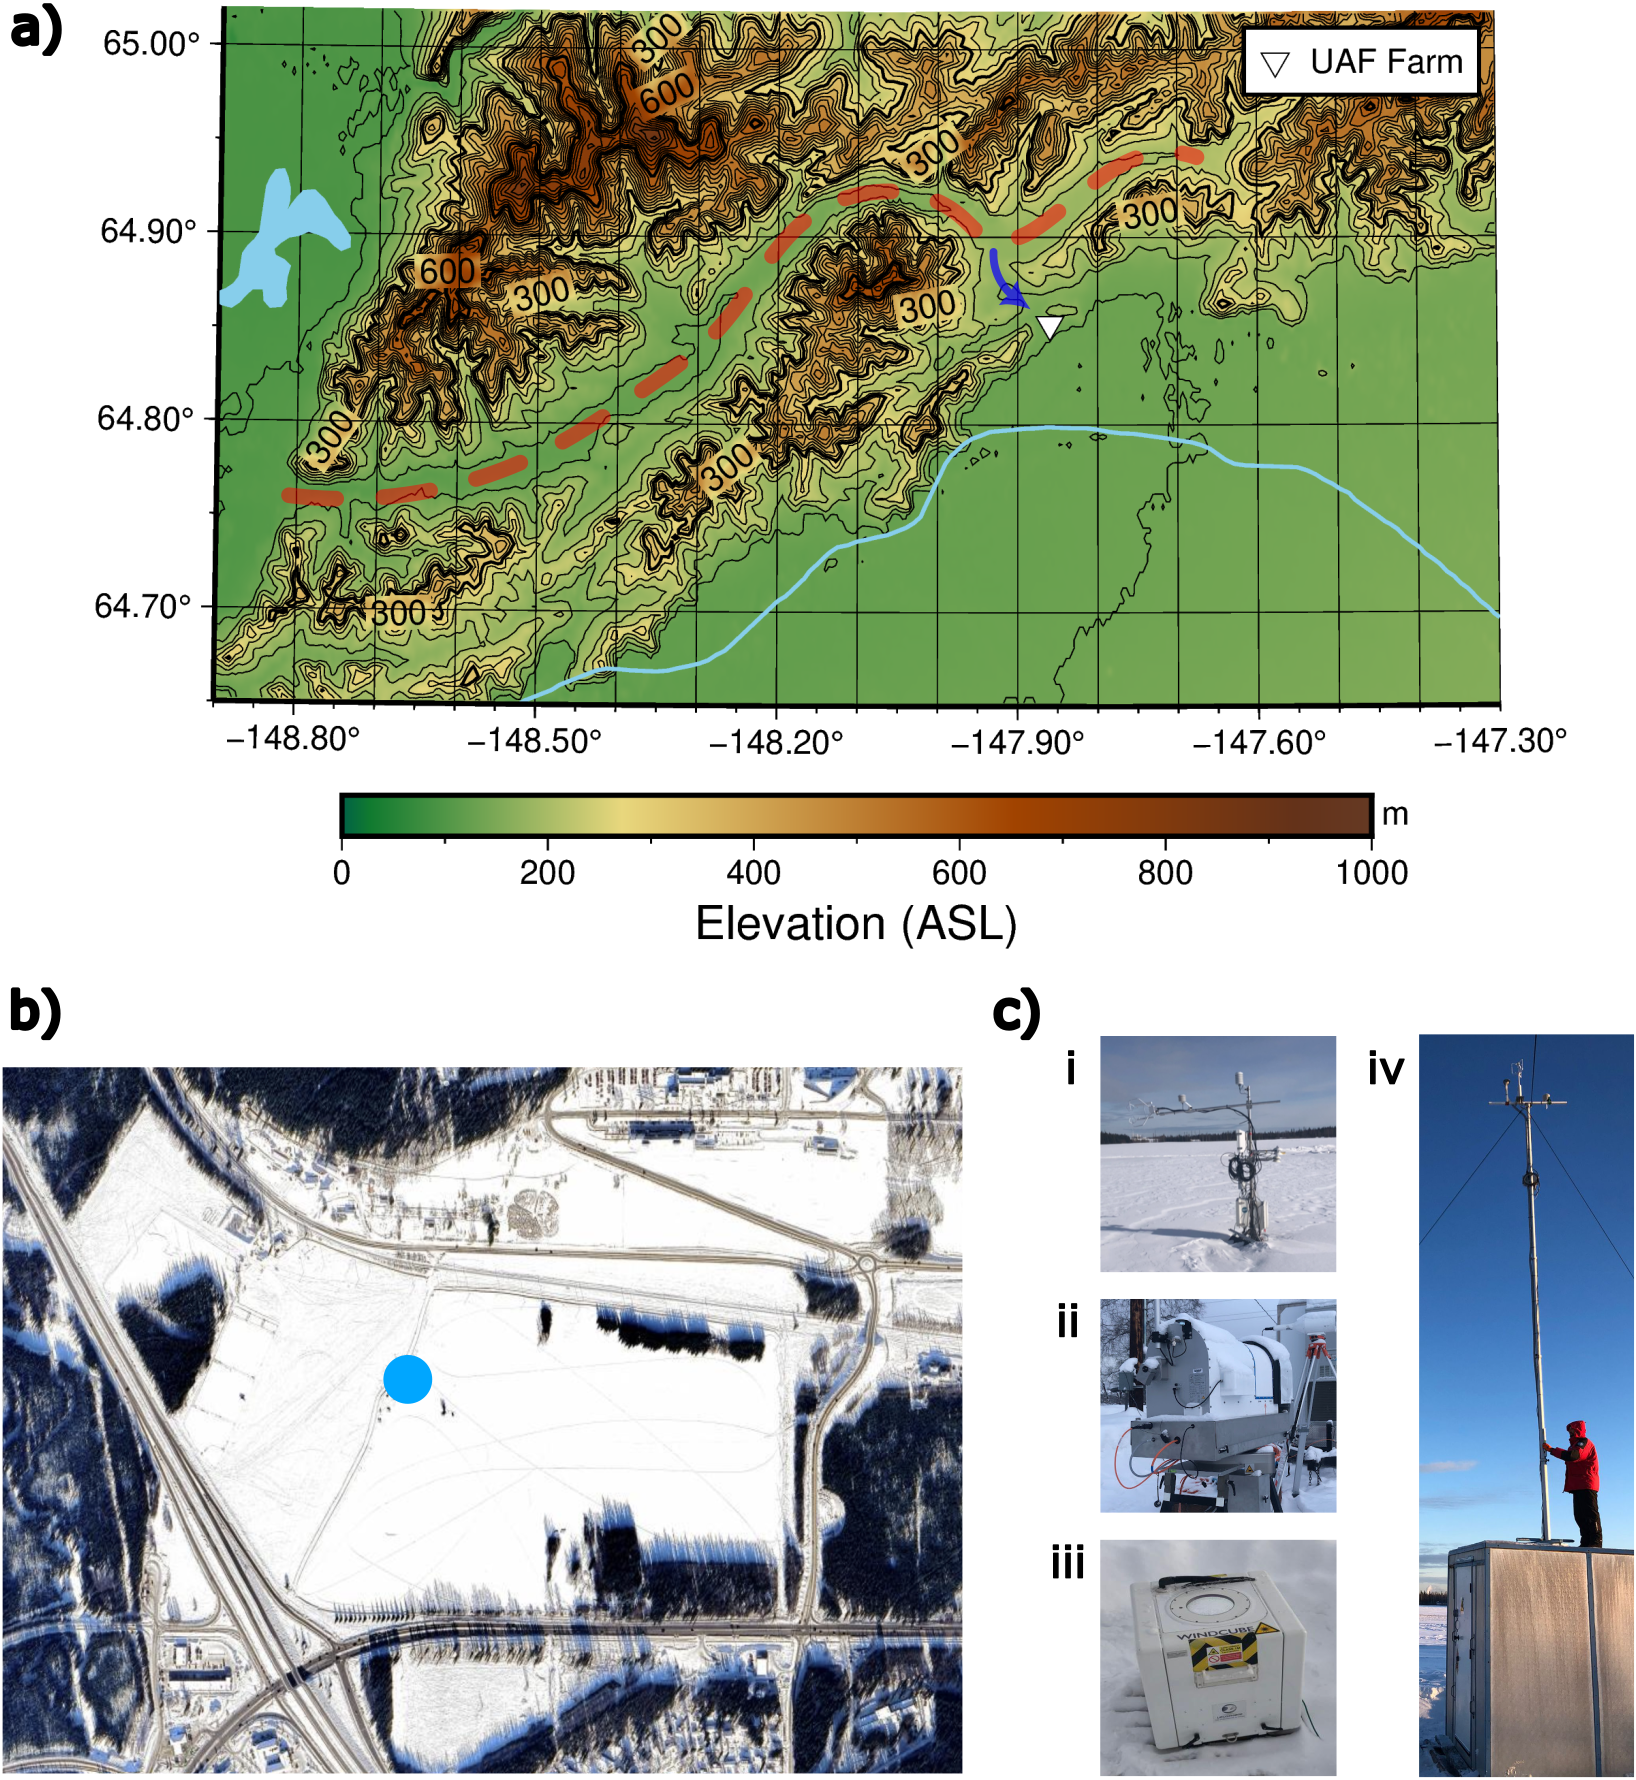
\includegraphics{../figures/instruments.png}
\caption{a) is the region. b) is the UAF Farm and instrument location. c) and its subparts are the instruments presented.}
\label{fig1}     
\end{figure}


%  ══════════════════════════════════════════════════════════════════════════
% instruments
%  ══════════════════════════════════════════════════════════════════════════

\section{Instrumentation and Methods}
\label{sec:methods}


One tower was set at 3 meter height to capture 3 component velocity through the 



%  ══════════════════════════════════════════════════════════════════════════
% results
%  ══════════════════════════════════════════════════════════════════════════

\section{Results and Discussion}
\label{sec:res_disc}


\subsection{Synoptic Conditions}


%  ══════════════════════════════════════════════════════════════════════════
% conclusion
%  ══════════════════════════════════════════════════════════════════════════

\section{Conclusion}
\label{sec:conclusion}


%  ══════════════════════════════════════════════════════════════════════════
% acknowledgements
%  ══════════════════════════════════════════════════════════════════════════

\begin{acknowledgements}
These should follow the concluding section of the paper and precede the References and any appendices, if they are present. The acknowledgements section does not require a section number. 
\end{acknowledgements} 


%  ══════════════════════════════════════════════════════════════════════════
% appendix
%  ══════════════════════════════════════════════════════════════════════════

%\section*{Appendix 1: Title of Appendix}
%\{Appendices are optional, as are appendix titles\}\\
%Appendices should precede the references and should be numbered (if there is more than one appendix). Equations, tables, and figures contained within the appendices should be numbered sequentially following those in the main text.


%  ══════════════════════════════════════════════════════════════════════════
% bibliography
%  ══════════════════════════════════════════════════════════════════════════

\bibliographystyle{spbasic_updated}     
\bibliography{main} 


%  ══════════════════════════════════════════════════════════════════════════
% SI
%  ══════════════════════════════════════════════════════════════════════════

%\newpage

%\section*{Supplementary Material for \textit{Boundary-Layer Meteorology} Sample Paper: Instructions for Authors}

%{\textbf{First Author* $\cdot$ Second Author $\cdot$ Third Author \\}}
%\\
%\text{*}Affiliation and email address for the corresponding author only (note that the corresponding author does not need to be the first author).

%\section*{1 Supplementary Electronic Materials}
%Supplementary multimedia files and other supplementary materials are also accepted for online publication in \textit{Boundary-Layer Meteorology }alongside an article. The supplementary files should be provided in standard file formats.

%To accommodate user downloads, please keep in mind that larger-sized files may require very long download times and that some users may experience other problems during downloading.

%\subsection*{1.1 Audio, Video, and Animations}
%Video and animation files should be provided at an aspect ratio of 16:9 or 4:3. The maximum file size that can be accommodated is 25 GB. The minimum allowable video length is 1 s. The supported file formats include avi, wmv, mp4, mov, m2p, mp2, mpg, mpeg, flv, mxf, mts, m4v, and 3gp. Video files should not contain more than three flashes per second.

%\subsection*{1.2 Presentations, Text Files, and Spreadsheets}
%Supplemental text files and presentations should be submitted as pdf files. Files in doc or ppt format cannot be accepted. Spreadsheets should also be converted to pdf format if they are intended for viewing only. If readers are encouraged to download and use the spreadsheet, then it can be provided in xls format.

%\subsection*{1.3 Specialized Formats}
%Other specialized file formats can also be supplied (e.g., tex, pdb, wrl, nb). It is also possible to provide multiple files within a zip or gz file.

%\section*{2 General Information}
%All supplementary materials should be specifically cited within the main text of the manuscript, in a manner similar to citing tables and figures. The supplementary materials should be cited as ``Online Resource", e.g., ``... as shown in the animation (Online Resource 3)", ``... additional data are provided in Online Resource 4". If more than one supplementary file is provided, these files should be numbered sequentially following the order they are cited in the main text, e.g., ``ESM\_1.mpg", ``ESM\_2.avi". Each supplementary file also requires a concise caption that describes the contents of the file. These captions should be listed at the end of the manuscript at initial submission.

%Authors should note that supplementary materials will be published without any conversion, editing, or reformatting. 
%\clearpage

\end{document}

